In dit hoofdstuk worden de verschillende lasten van de moonrover berekend. In de formules word er een hellingshoek aan gehouden van 0 graden. De bescreven fomrules zijn allemaal voor 1 wiel. Voor de gehele moonrover zal dit dus x4 moeten. In de afbeeldingen is ook te zijn hoe de eigenschappen zich gedragen onder diverse hellingshoeken.

\subsection{Rollast}
    Rollast is de last die minaal overwonnen moet worden een wiel te laten draaien. Dit verschilt ook onder welke hellingshoek de moonrover staat. In afbeelding \ref{fig:birds} is te zien hoe de rolllast veranderd onder diverse hellingshoeken.

    \begin{figure}[H]
        \centering
        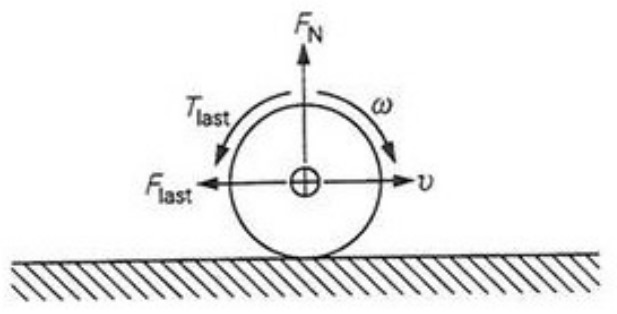
\includegraphics[scale=0.5]{Rolweerstand.jpg}
        \caption{rollast krachten}
    \end{figure}

    \begin{multicols}{2}
        \textbf{Formules:}
        \begin{equation}
            \begin{split}
                T_{last} &= f_{rol} \cdot F_{N} \cdot r \\
                F_{N} &= m \cdot g \cdot cos(\alpha) \\
                &\Downarrow \\
                T_{last} &= 0.1 \cdot 2.43 \cdot 0.075 = 18.23 [mNm]
            \end{split}
        \end{equation}

        \textbf{constante:}
        \begin{equation*}
            \begin{split}
                f_{rol} &= 0,1 \\
                r &= 0,075 [m] \\
                m &= 1,5 [N] \\
                g &= 1,62 [m/s^2] \\
                \alpha &= 0^\circ
            \end{split}
        \end{equation*}
    \end{multicols}

\subsection{Hellingslast}
    Hellingslast is de last die om de hoek komt kijken zodra de moonrover zich onder een helling bevindt. Wanneer deze helling stijgend is zal dit de last zijn die overtroffen moet worden om voorruit te komen. Wanneer deze helling dalend is is dit de last die overtroffen moet worden of tot stilstand te komen.

    \begin{figure}[H]
        \centering
        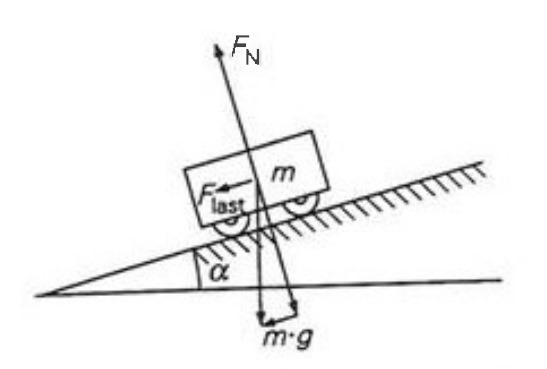
\includegraphics[scale=0.5]{Hellingsweerstand.jpg}
        \caption{hellinglast krachten}
    \end{figure}

    \begin{multicols}{2}
        \textbf{Formules:}
        \begin{equation}
            \begin{split}
                T_{last} &= f_{Z} \cdot sin(\alpha) \cdot r \\
                F_{Z} &= m \cdot g\\
                &\Downarrow \\
                T_{last} &= 2.43 \cdot 0 \cdot 0.075 = 0 [mNm]
            \end{split}
        \end{equation}

        \textbf{constante:}
        \begin{equation*}
            \begin{split}
                r &= 0,075 [m] \\
                m &= 1,5 [N] \\
                g &= 1,62 [m/s^2] \\
                \alpha &= 0^\circ 
            \end{split}
        \end{equation*}
    \end{multicols}

    \begin{figure}[H]
        \centering
        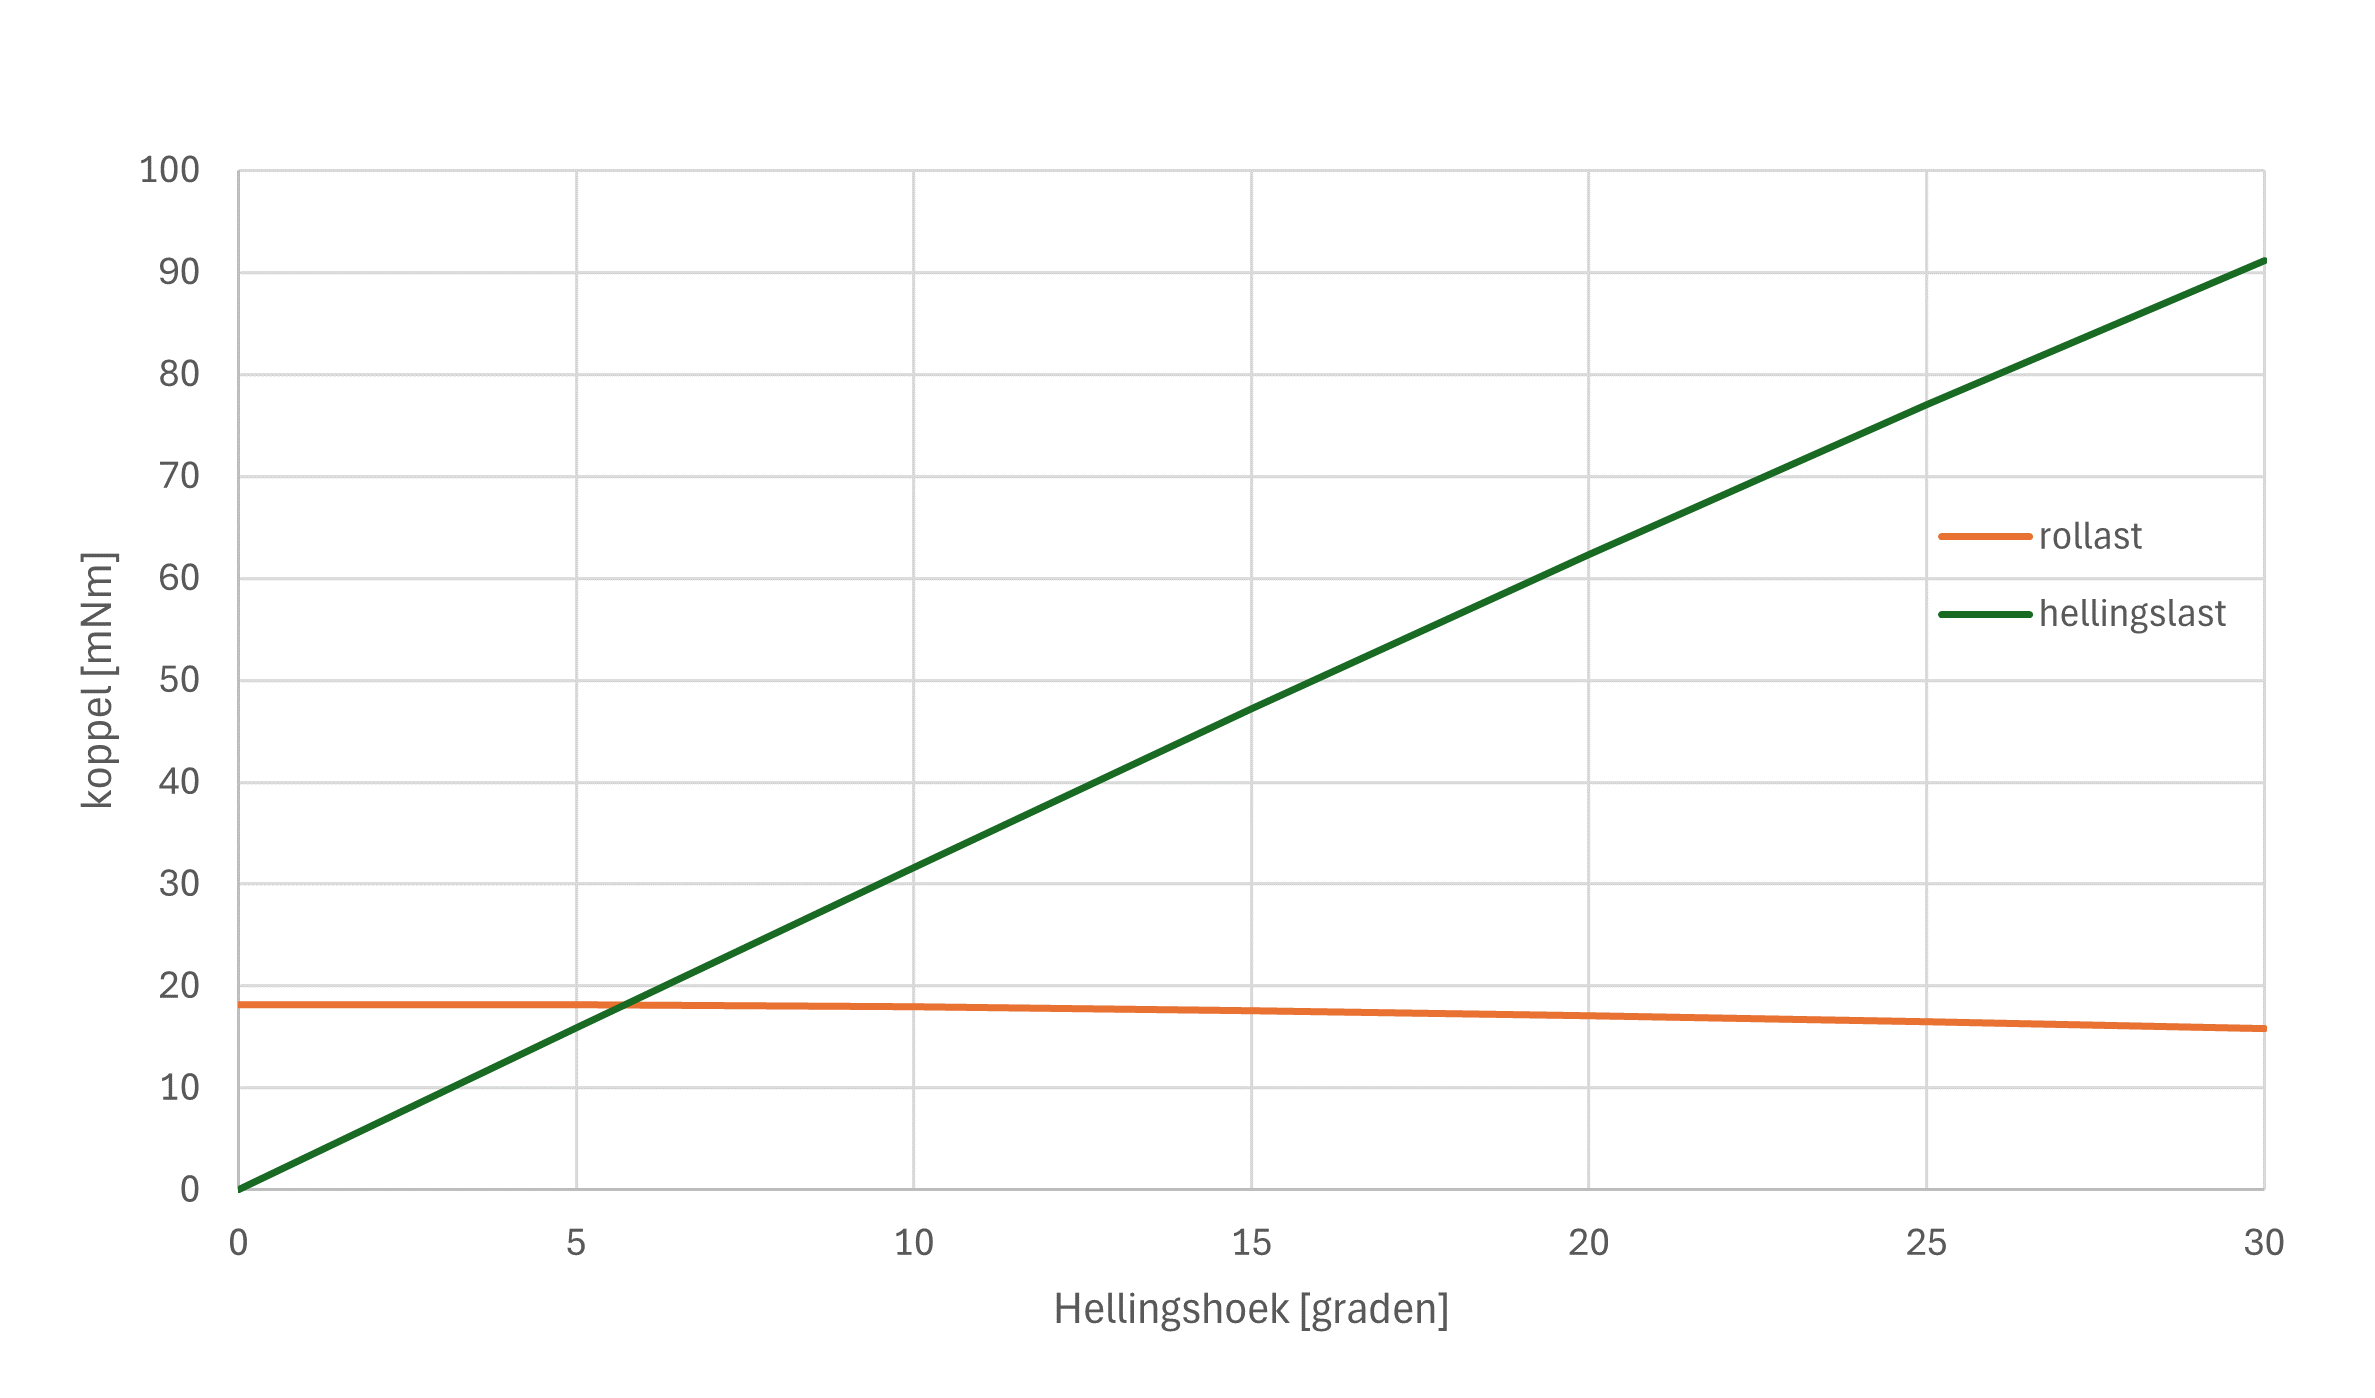
\includegraphics[scale=0.7]{rolkoppel_NEW.png}
        \caption{rolweerstand vs hellingsweerstand onder verschillende hoeken}
        \label{fig:birds}
    \end{figure}

    In figuur \ref{fig:birds} is te zien hoe de rolweerstand en de hellingsweerstand zich gedragen ten opzichte van verschillende hellingshoeken. In de grafiek is te zien dat vanaf een hoek $\approx 5.7^\circ$ de moonrover altijd stil zal blijven staan. Dit komt doordat de moonrover tot dit punt nog niet voorbij zijn rollast komt. Het snijpunt van de rollast met de hellingslast wordt als volgt berkent:
    \begin{equation}
        \begin{split}
            T_{rollast} &= T_{hellingslast} \\
            f_{rol} \cdot F_{N} \cdot r &= F_{N} \cdot sin(\alpha) \cdot r \\
            f_{rol} &= sin(\alpha) \\
            0.1 &= sin(\alpha) \\
            \alpha &= sin-1(0.1) \\
            \alpha &= 5.72^\circ
        \end{split}
    \end{equation}

\subsection{Grip}
    Onder grip verstaan we de hoeveelheid koppel die op de aandrijving gegeven kan worden zonder dat het wiel zal gaan slippen. Hierbij berkenen we dus ook wat het maximale koppel is die gegeven kan worden op de aandrijving.

    \begin{multicols}{2}
        \textbf{Formules:}
        \begin{equation}
            \begin{split}
                T_{max} &= \mu \omega \cdot F_{N} \cdot r \\
                F_{N} &= m \cdot g \cdot cos(\alpha) \\
                &\Downarrow \\
                T_{max} &= 0.9 \cdot 2.43 \cdot 0.075 = 164.03 [mNm]
            \end{split}
        \end{equation}

        \textbf{constante:}
        \begin{equation*}
            \begin{split}
                \mu \omega &= 0.9 \\
                r &= 0,075 [m] \\
                m &= 1,5 [N] \\
                g &= 1,62 [m/s^2] \\
                \alpha &= 0^\circ 
            \end{split}
        \end{equation*}
    \end{multicols}

    \begin{figure}[H]
        \centering
        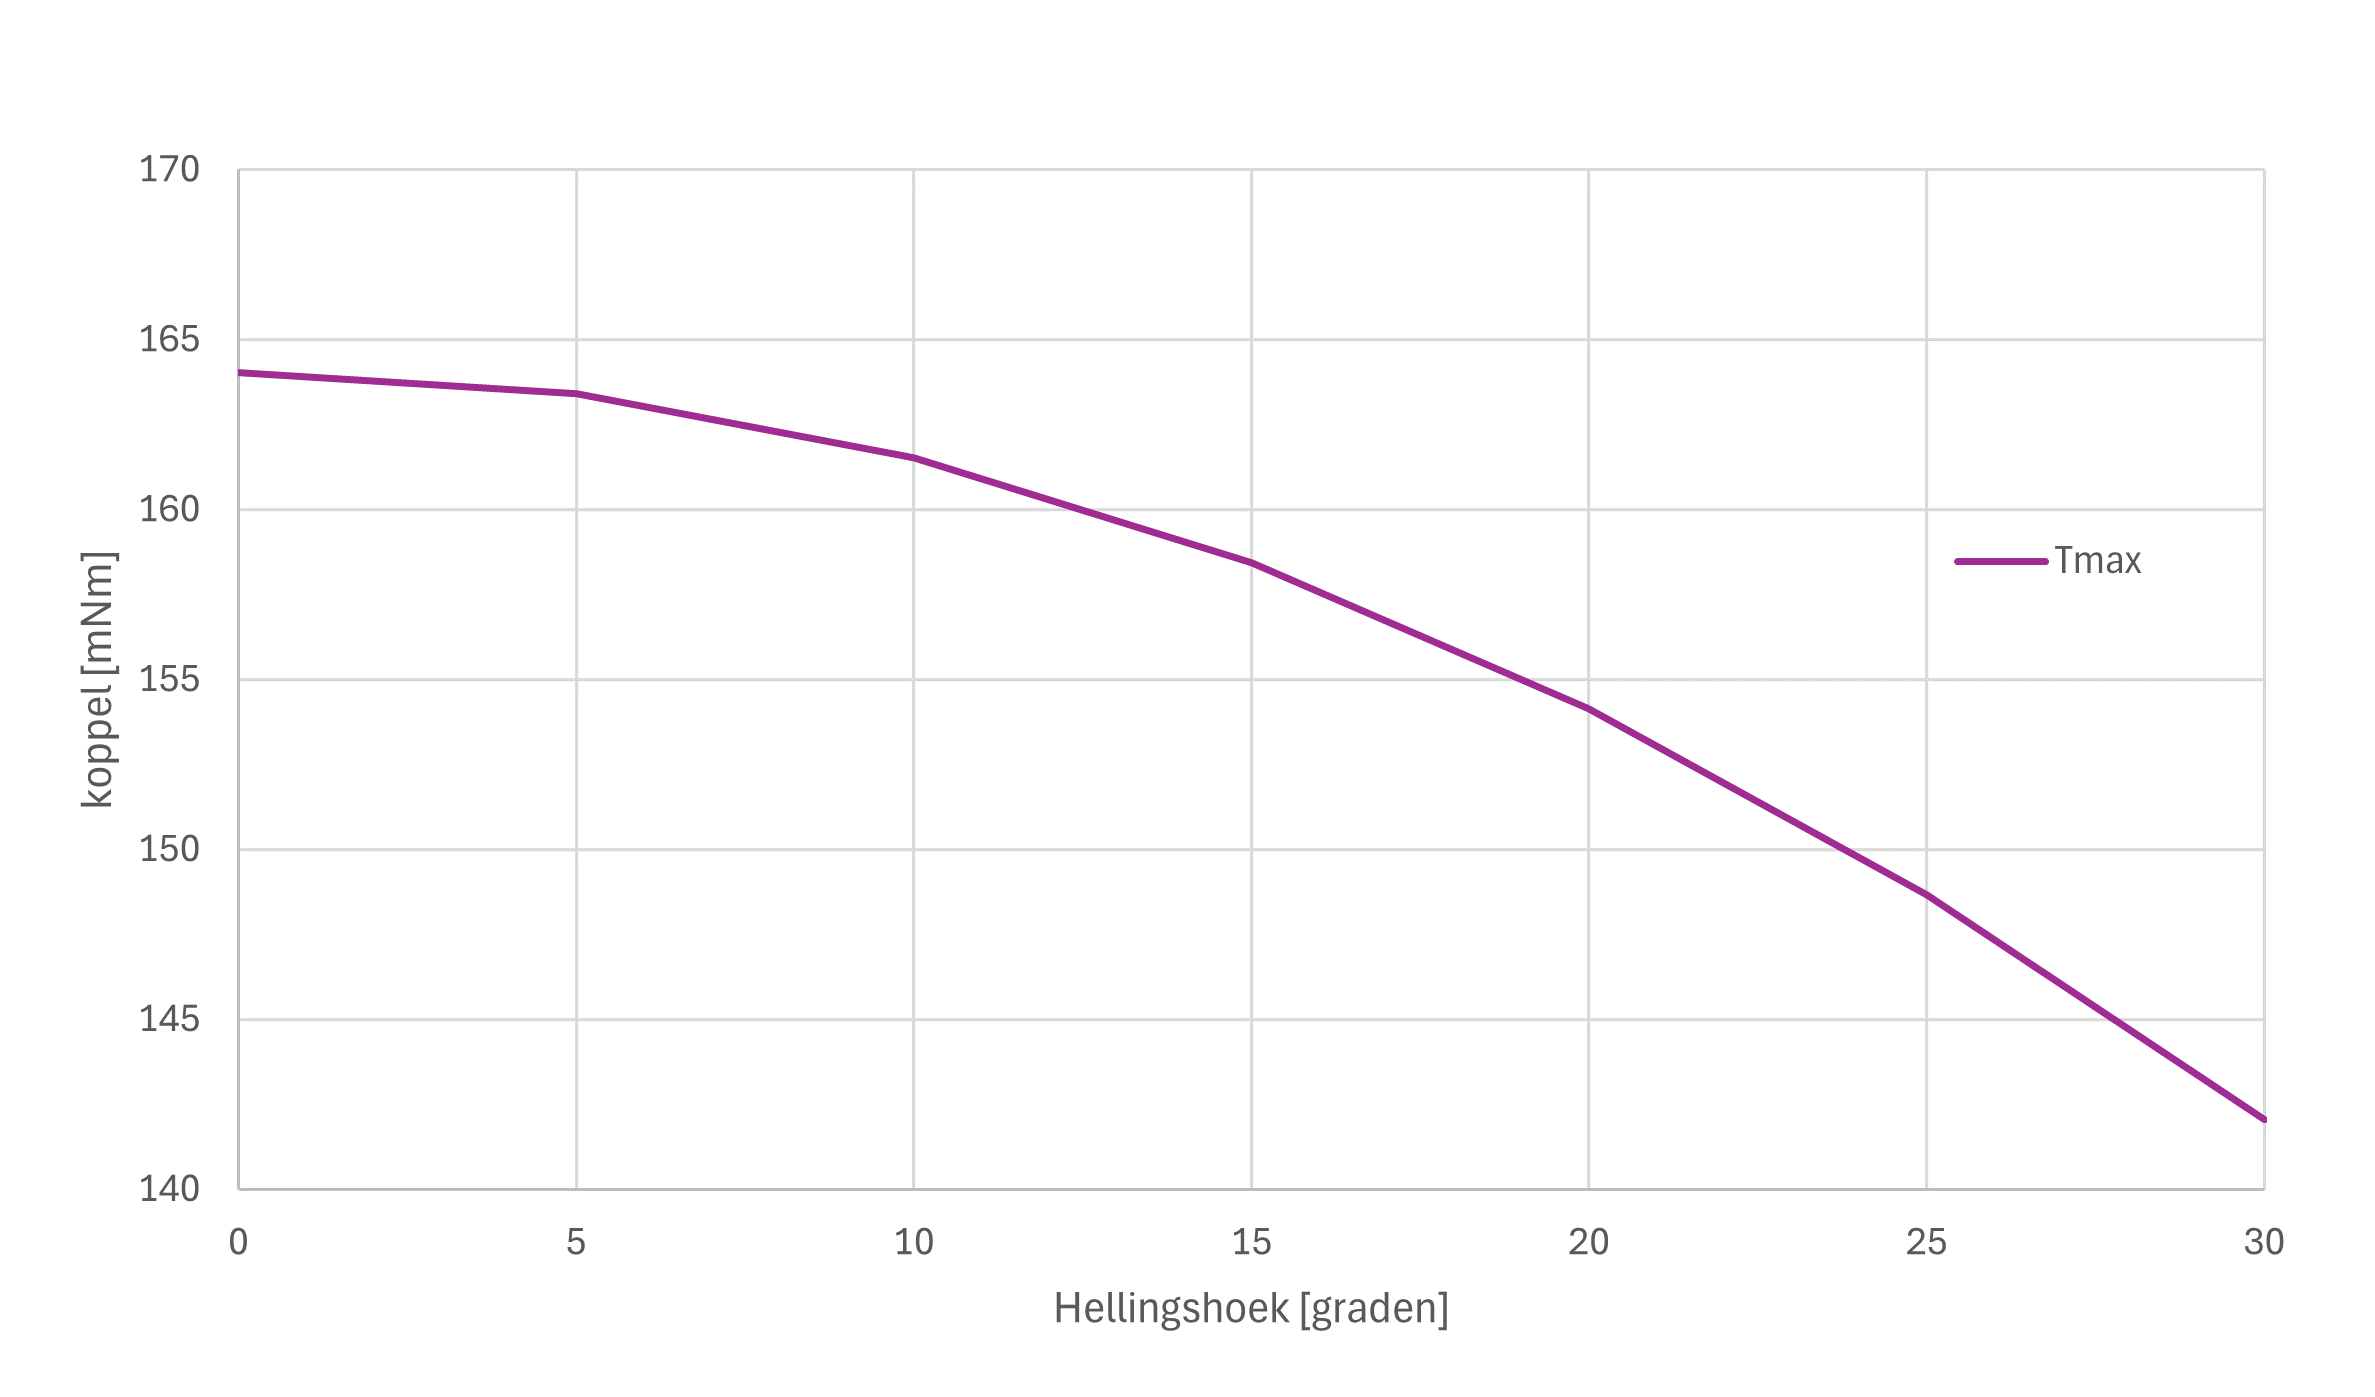
\includegraphics[scale=0.7]{maximumkoppel_NEW.png}
        \caption{$T_{max}$}
        \label{fig:peanut}
    \end{figure}

    In figuur \ref{fig:peanut} is te zien hoe de maximale koppel zich weerhoud tegen de hellingshoek. Hierbij is duidelijk te zien dat de maximale koppel af neemt naarmate de hellingshoek groter wordt.

\subsection{Versnelling}
    Hier wordt het koppeloverschot berkend wat nodig is om de beoogde versnelling te behalen. 

    \begin{multicols}{2}
        \textbf{Formules:}
        \begin{equation}
            \begin{split}
                T_{acc} &= J \cdot \frac{d \omega}{dt} \\
                omtrek_{wiel} &= 2 \cdot \pi \cdot r = 0.47 [m] \\
                Versnelling &= \frac{a}{omtrek_{wiel}} = 1.49 [omwentelingen/s^2] \\
                &= 9.36 [rad/s^2] \\
                &\Downarrow \\
                T_{acc} &= 2.1 \cdot 10^{-3} \cdot 9.36 = 19.6 [mNm]\\
            \end{split}
        \end{equation}

        \textbf{constante:}
        \begin{equation*}
            \begin{split}
                a &= 0.7 [m/s^2] \\
                J &= 2.1 \cdot 10^{-3} [kg \cdot m^2]\\
                r &= 0,075 [m] \\
                m &= 1,5 [N] \\
                g &= 1,62 [m/s^2] \\
                \alpha &= 0^\circ 
            \end{split}
        \end{equation*}
    \end{multicols}

\subsection{Snelheid}
    Hier berkenen we de maximale rpm waarbij de maximale snelheid van van 2.1 m/s niet word overtroffen.

    \begin{multicols}{2}
        \textbf{Formules:}
        \begin{equation}
            \begin{split}
                omtrek &= 2 \cdot \pi \cdot r \\
                snelheid &= \frac{speed_{max}}{omtrek}\ = \frac{2.1}{0.47} = 4.46 [omw/s]\\
                &\Downarrow \\
                 &= 267.4 [rpm]
            \end{split}
        \end{equation}

        \textbf{constante:}
        \begin{equation*}
            \begin{split}
                speed_{max} &= 2.1 [m/s]\\
                r &= 0,075 [m] 
            \end{split}
        \end{equation*}
    \end{multicols}

\newpage

\subsection{Conclusie}
In dit hoofdstuk heb je kunnen lezen hoe we de lasten van de moonrover hebben bepaald. Dit was nodig om een geschikte motor te kunnen selecteren voor de moonrover.  In afbeelding \ref{fig:lasten moonrover} is het werkgebied te zien van de moonrover doormiddel van de rode lijnen. In het volgnende hoofdstuk zal er een geschikte motor en transmissie geselecteerd worden die juist aansluit bij deze last. 

\begin{figure}[H]
    \centering
    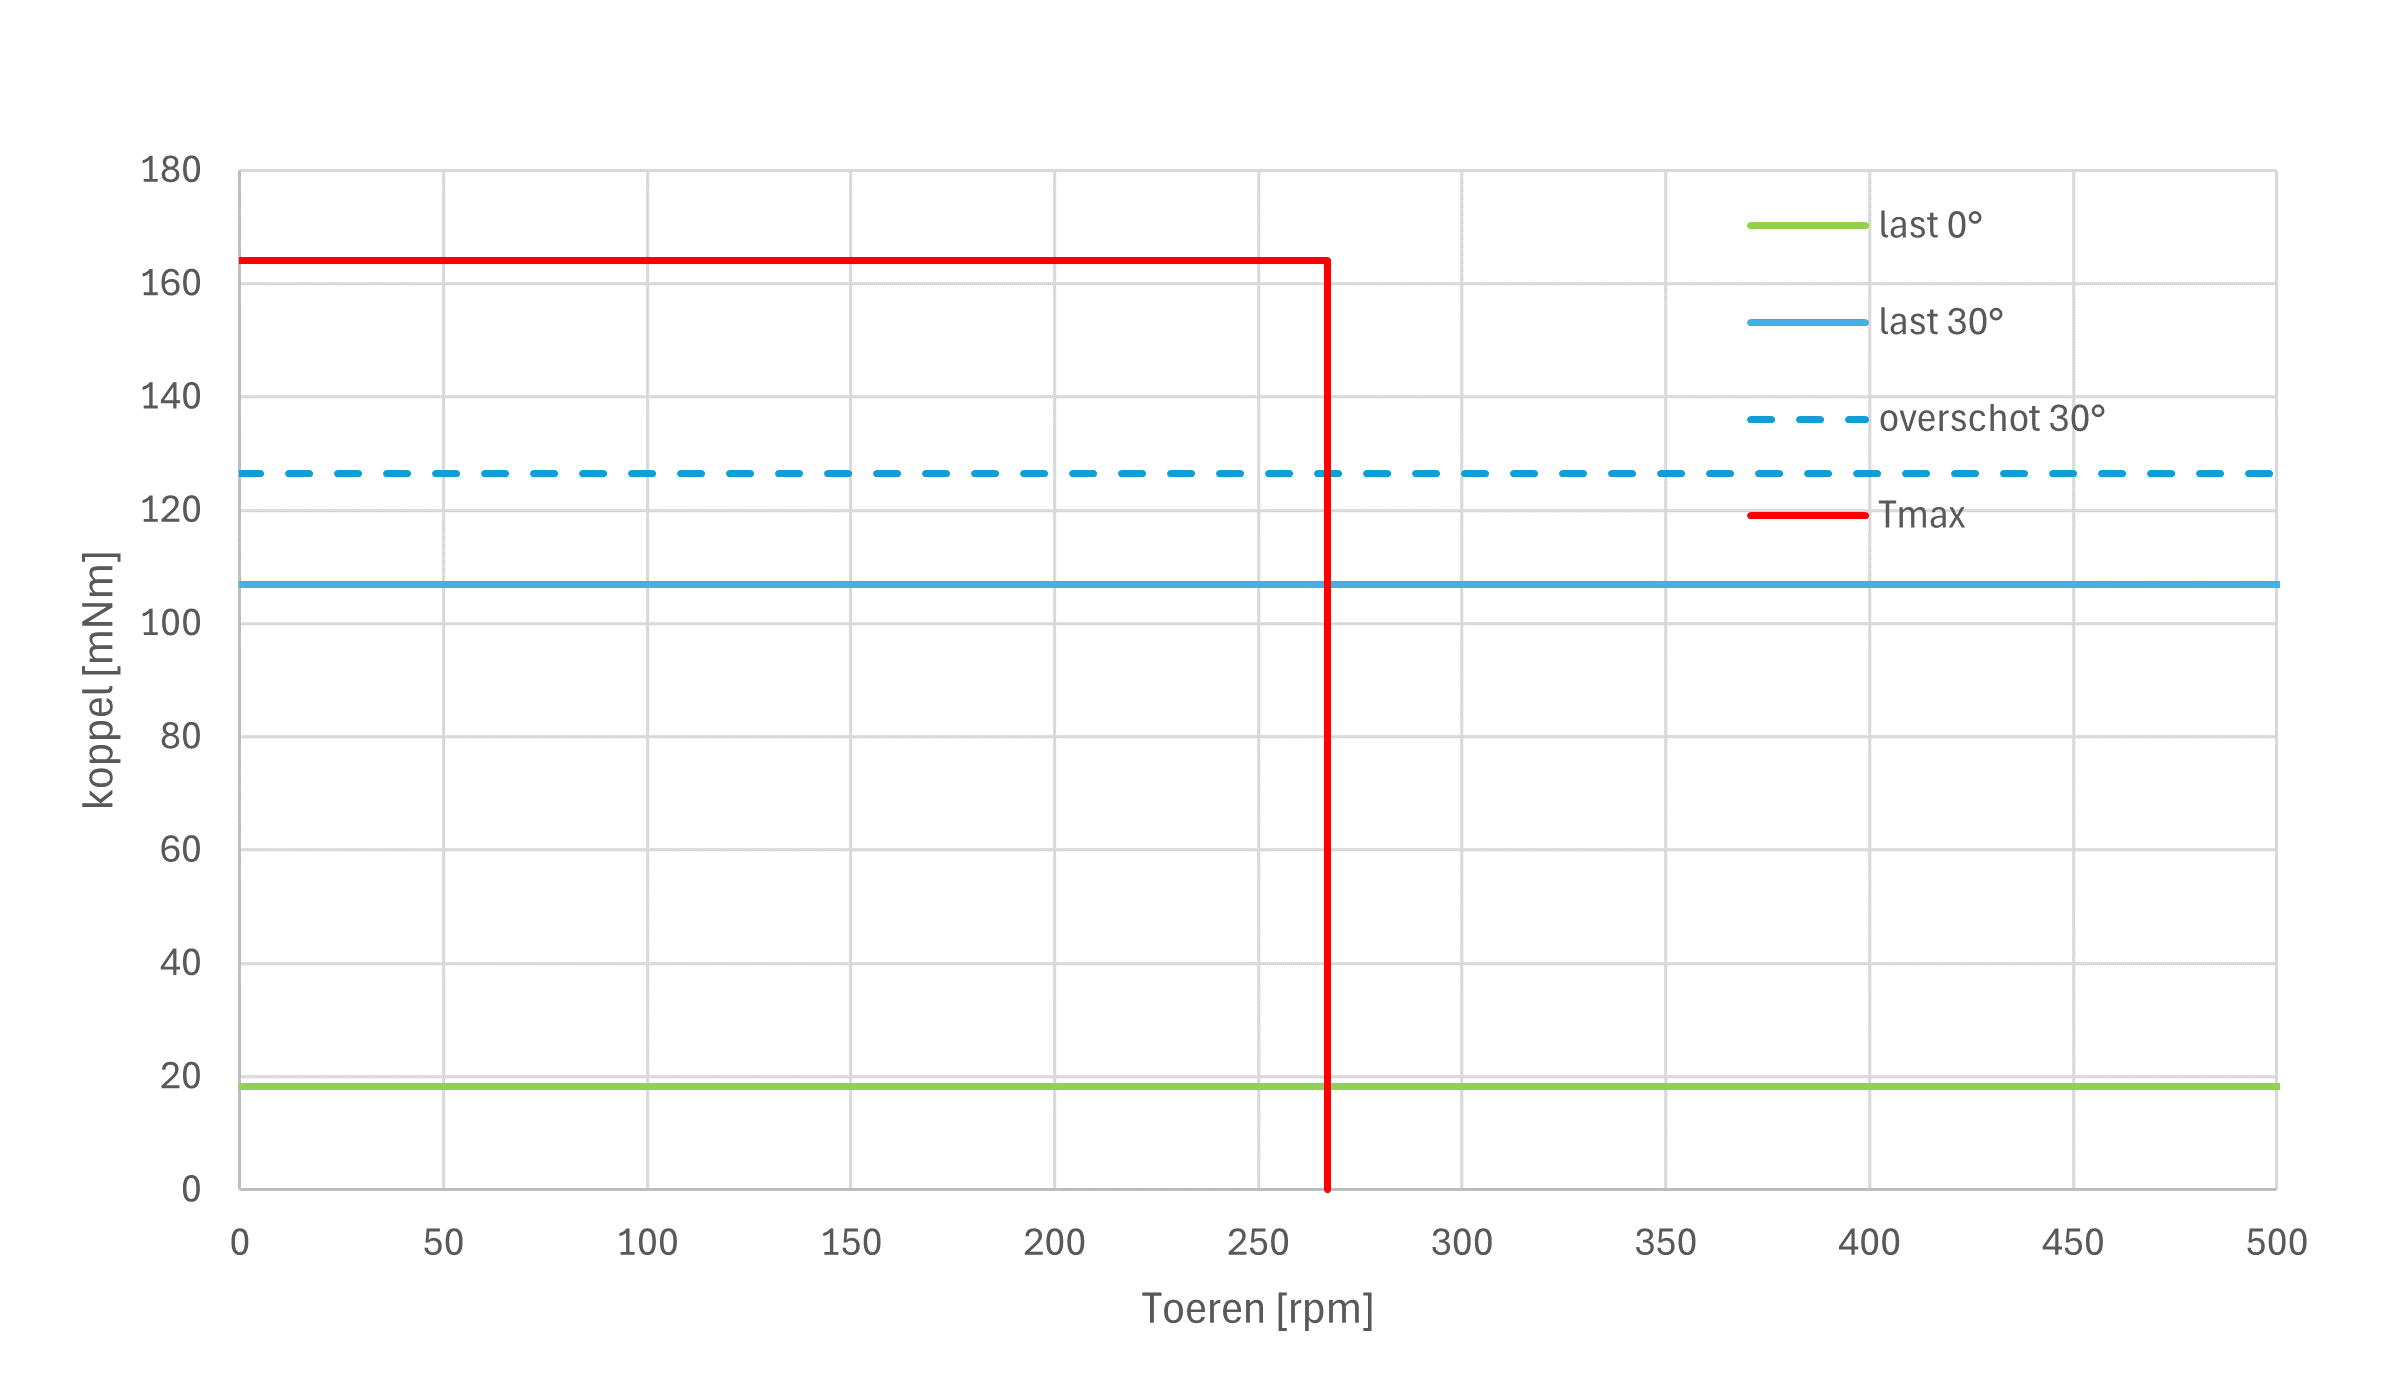
\includegraphics[scale=0.7]{lastkoppel_NEW.png}
    \caption{Lasten moonrover}
    \label{fig:lasten moonrover}
\end{figure}
    
